%-------------------------------------------------------------------------------
%-------------------------------------------------------------------------------
%-------------------------------------------------------------------------------
\chapter{Fonctions}
%-------------------------------------------------------------------------------
%-------------------------------------------------------------------------------
\thispagestyle{empty}
%-------------------------------------------------------------------------------
%-------------------------------------------------------------------------------
\begin{abstract} Dans ce T.P. nous allons utiliser des fonctions utiles de python, définir les premières fonctions et utiliser les instructions de branchement.

Dans un premier temps on donnera un cadre de présentation du code écrit dans l'éditeur qu'il conviendra de respecter à chaque T.P.
\end{abstract}
%-------------------------------------------------------------------------------
%-------------------------------------------------------------------------------
%-------------------------------------------------------------------------------
\section{Mise en page dans l'éditeur} 
%-------------------------------------------------------------------------------
%-------------------------------------------------------------------------------
%-------------------------------------------------------------------------------
Dans les T.P. nous importerons des fonctions définis dans des modules, nous définirons nos propres fonctions et nous utiliserons ces fonctions pour obtenir des résultats. 

Il est utile de structurer le code écrit. Pour cela chaque T.P. on commencera donc par indiquer, par un commentaire, les parties selon la forme ci-dessous.

\begin{lstlisting}
## Importations



## Fonctions



## Principal



\end{lstlisting}
\begin{description}
  \item[Importations] est l'endroit où on importe les modules, par exemple
\type{from math import *}

C'est aussi ici que l'on pourra charger des fichiers et définir des constantes

  \item[Fonctions] est l'endroit où on écrit les fonctions.
  
  \item[Principal] est l'endroit où on écrit les scripts qui utilisent les fonctions.
\end{description}
%-------------------------------------------------------------------------------
%-------------------------------------------------------------------------------
%-------------------------------------------------------------------------------
\section{Vers des fonctions utiles} 
%-------------------------------------------------------------------------------
%-------------------------------------------------------------------------------
%-------------------------------------------------------------------------------
On cherche à écrire une fonction qui calcule l’hypoténuse d'un triangle rectangle à partir des longueurs des côtés.
\begin{center}
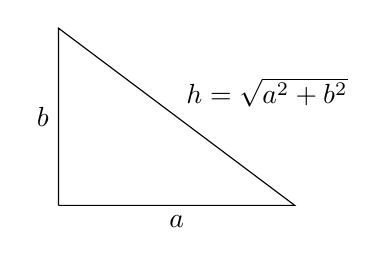
\begin{tikzpicture}[scale = 0.75]
\draw (0,0) -- node[below] {$a$} (4, 0) -- node[above right] {$h = \sqrt{a^2+b^2}$} (0, 3) -- node[left] {$b$} (0, 0);
\end{tikzpicture}
\end{center}
%-------------------------------------------------------------------------------
%-------------------------------------------------------------------------------
\subsection{Un calcul vain} 
%-------------------------------------------------------------------------------
%-------------------------------------------------------------------------------
Jules Jefonce écrit la fonction suivante 
%-------------------------------------------------------------------------------
\begin{lstlisting}
def hypo1(a, b):
    """Entrées : deux nombres
       Sortie : l'hypothénuse du triangle rectangle de cotes a et b"""
    (a**2 + b**2)**0.5
\end{lstlisting}
%-------------------------------------------------------------------------------
%-------------------------------------------------------------------------------
\begin{Exercise}
\it Peut-on obtenir le résultat de \type{hypo1(4, 7)} ?

On pourra essayer \type{print(hypo1(4, 7))} dans la partie principale et \type{hypo1(4, 7)} dans la console.
\end{Exercise}
%-------------------------------------------------------------------------------
\begin{Answer}
Rien ne marche, on voit apparaître des \type{None}.
\end{Answer} 
%-------------------------------------------------------------------------------
%-------------------------------------------------------------------------------

\medskip

Jules se souvient que les résultats sont perdus si on ne les mémorisent pas dans une variable ; il écrit alors
%-------------------------------------------------------------------------------
\begin{lstlisting}
def hypo2(a, b):
    """Entrées : deux nombres
       Sortie : l'hypothénuse du traingle rectangle de cotes a et b"""
    h = (a**2 + b**2)**0.5
\end{lstlisting}
%-------------------------------------------------------------------------------
%-------------------------------------------------------------------------------
\begin{Exercise}
\it La variable \type{h} est-elle accessible après le calcul de \type{hypo2(4, 7)} ?

Vérifier dans le Workspace de Pyzo ou l'onglet des variables de Thonny.
\end{Exercise}
%-------------------------------------------------------------------------------
\begin{Answer}
 \type{h} a disparu
\end{Answer} 
%-------------------------------------------------------------------------------
%-------------------------------------------------------------------------------
\subsection{Voir le résultat} 
%-------------------------------------------------------------------------------
%-------------------------------------------------------------------------------
Sandrine Lafutée, la voisine de Jules, lui dit, "C'est normal, tout ce qui est dans la fonction est oublié, il faut afficher le résultat depuis la fonction".

Cette entraide leur permet d'écrire
%-------------------------------------------------------------------------------
\begin{lstlisting}
def hypo3(a, b):
    """Entrées : deux nombres
       Sortie : l'hypothénuse du traingle rectangle de cotes a et b"""
    h = (a**2 + b**2)**0.5
    print(h)
\end{lstlisting}
%-------------------------------------------------------------------------------
Ils essayent leur fonction en écrivant \type{hypo3(4, 7)} et ça marche.
%-------------------------------------------------------------------------------
%-------------------------------------------------------------------------------
\begin{Exercise}
\it On utilise la fonction dans la partie principale : \type{print(hypo3(4, 7))}.

Est-ce le résultat attendu ?
\end{Exercise}
%-------------------------------------------------------------------------------
\begin{Answer}
En plus du résultat, on voit apparaître un \type{None}
\end{Answer} 
%-------------------------------------------------------------------------------
%-------------------------------------------------------------------------------
\subsection{Utiliser le résultat} 
%-------------------------------------------------------------------------------
%-------------------------------------------------------------------------------
Ils passent outre le petit souci précédent et passent à la question suivante : il faut tester si 5, 12 et 13 sont les côtés d'un triangle rectangle. Ils écrivent donc le test dans la console et obtiennent\footnote{Python est laxiste ici, il ne devrait pas indiquer \type{False} mais renvoyer une erreur.}
%-------------------------------------------------------------------------------
\begin{lstlisting}
>>> hypo3(5, 12) == 13
13
False
\end{lstlisting}
%-------------------------------------------------------------------------------
%-------------------------------------------------------------------------------
\begin{Exercise}
\it Écrire une fonction \type{hypo4} qui peut être utilisée.
\end{Exercise}
%-------------------------------------------------------------------------------
\begin{Answer}
\begin{lstlisting}
def hypo4(a, b):
    """Entrées : deux nombres
       Sortie : l'hypothénuse du traingle rectangle de cotes a et b"""
    h = (a**2 + b**2)**0.5
    return h
\end{lstlisting}
\end{Answer} 
%-------------------------------------------------------------------------------
%-------------------------------------------------------------------------------

\medskip

Moralité : {\bf si on demande de renvoyer un résultat, on le renvoie avec \Type{return}}.
%-------------------------------------------------------------------------------
%-------------------------------------------------------------------------------
%-------------------------------------------------------------------------------
\section{Fonctions} 
%-------------------------------------------------------------------------------
%-------------------------------------------------------------------------------
%-------------------------------------------------------------------------------
\subsection{Fonctions simples} 
%-------------------------------------------------------------------------------
%-------------------------------------------------------------------------------
\begin{Exercise}[title={Polynôme},label=exo:poly]
\it Écrire une fonction \type{P} telle que \type{P(a)} renvoie la valeur du polynôme $X^3-7.2 X + 1.4$ en $a$.
\end{Exercise}
%-------------------------------------------------------------------------------
\begin{Answer}
\begin{lstlisting}
def P(x):
    return x**3 - 7.2*x + 1.4
\end{lstlisting}
\end{Answer} 
%-------------------------------------------------------------------------------
%-------------------------------------------------------------------------------
\begin{Exercise}[title={Maximum}]
\it La fonction \type{max} renvoie le maximum de 2 nombres.

Écrire une fonction \type{max3} renvoyant le plus grand parmi $3$ nombres. 
\end{Exercise}
%-------------------------------------------------------------------------------
\begin{Answer}
\begin{lstlisting}
def max3(x, y, z):
    a = max(x, y) 
    return max (a, z)
\end{lstlisting}
\end{Answer} 
%-------------------------------------------------------------------------------
%-------------------------------------------------------------------------------
\begin{Exercise}[title={Devinette}]
\it Importer le module \type{math} afin de pouvoir utiliser la constante \type{pi} et la fonction \type{floor}.

Tester la fonction suivante pour \type{nombre = pi} et \type{n = 1}, \type{n = 2}, \type{n = 3}.
\begin{lstlisting}
def devine(nombre, n):
    a = 10**(n-1)*nombre
    b = a - floor(a)
    return floor(10*b)
\end{lstlisting}
Que fait cette fonction?
\end{Exercise} 
%-------------------------------------------------------------------------------
\begin{Answer}
Elle calcule la $n$-ième décimale du nombre.
\end{Answer} 
%-------------------------------------------------------------------------------
%-------------------------------------------------------------------------------
\medskip
Une fonction déjà écrite peut bien entendu être utilisée dans une fonction. 
%-------------------------------------------------------------------------------
%-------------------------------------------------------------------------------
\begin{Exercise}[title={Taux d'accroissement}, label = exo:accP]
\it Écrire une fonction \type{acc\_P(a, b)} qui renvoie le taux d'accroissement de $P$ entre $a$ et $b$ : $\displaystyle \frac{P(b) -P(a)}{b-a}$. $P$ est le polynôme défini à la question \ref{exo:poly}.
\end{Exercise}
%-------------------------------------------------------------------------------
\begin{Answer}
\begin{lstlisting}
def acc_P(a, b)):
    return (P(b) - P(a))/(b-a)
\end{lstlisting}
\end{Answer} 
%-------------------------------------------------------------------------------
%-------------------------------------------------------------------------------
\subsection{Résultats booléens} 
%-------------------------------------------------------------------------------
%-------------------------------------------------------------------------------
Lorsque l'on fait une comparaison, l'expression renvoie un booléen qui peut être retourné. Par exemple
%-------------------------------------------------------------------------------
\begin{lstlisting}
def est_positif(x):
    return x > 0
\end{lstlisting}
%-------------------------------------------------------------------------------
Les fonctions de cette partie doivent être écrites sans utiliser l'instruction conditionnelle \Type{if}.
%-------------------------------------------------------------------------------
%-------------------------------------------------------------------------------
\begin{Exercise}[title={Parité}]
\it Écrire une fonction \type{est\_pair} telle que \type{est\_pair(n)} renvoie \type{True} ou \type{False} selon que l'entier $n$ est pair ou impair.
\end{Exercise}
%-------------------------------------------------------------------------------
\begin{Answer}
\begin{lstlisting}
def est_pair(n):
    return n%2 == 0
\end{lstlisting}
\end{Answer} 
%-------------------------------------------------------------------------------
%-------------------------------------------------------------------------------
\begin{Exercise}[title={Intervalle}]
\it Écrire une fonction \type{entre} telle que \type{entre(a, b, x)} renvoie \type{True} ou \type{False} selon que le réel $x$ est appartient à l'intervalle $[a; b]$ ou non. La fonction {\bf ne doit pas} utiliser l'instruction \type{if}.

Remarque : {\sc Python} permet d'écrire la fonction sans utiliser \type{and}.
\end{Exercise}
%-------------------------------------------------------------------------------
\begin{Answer}
\begin{lstlisting}
def entre(a, b, x):
    return a <= x and x <= b
\end{lstlisting}

L'écriture suivante est possible 
\begin{lstlisting}
def entre(a, b, x):
    return a <= x <= b
\end{lstlisting}
\end{Answer} 
%-------------------------------------------------------------------------------
%-------------------------------------------------------------------------------
\medskip

Une année est {\bf bissextile}, c'est-à-dire qu'elle comporte 366 jours au lieu de 365 si elle est divisible par 4 sauf tous les centenaires (1700, 1800, 1900, ..). Cependant tous les multiples de 400 sont quand même bissextiles.
%-------------------------------------------------------------------------------
%-------------------------------------------------------------------------------
\begin{Exercise}[title={Années bissextiles}, label=exo:bissext1]
\it Écrire une fonction \type{bissextile(n)} qui renvoie \type{True} ou \type{False} selon que l'année $n$ est bissextile ou non.

On peut écrire une fonction sur 2 lignes : (\type{def} et \type{return}). 
\end{Exercise}
%-------------------------------------------------------------------------------
\begin{Answer}
\begin{lstlisting}
def bissextile(n):
    return (n%4 == 0 and n%100 != 0) or n%400 == 0
\end{lstlisting}
\end{Answer} 
%-------------------------------------------------------------------------------
%-------------------------------------------------------------------------------
%-------------------------------------------------------------------------------
\section{Paramètres} 
%-------------------------------------------------------------------------------
%-------------------------------------------------------------------------------
%-------------------------------------------------------------------------------
Un fonction peut ne pas avoir de variable : on peut écrire une fonction qui fait une suite constante d'instructions, on peut simuler un événement aléatoire, \dots

Le module \type{random} contient une fonction \type{randint} telle que \type{random.randint(a,b)} renvoie un entier choisi au hasard entre $a$ et $b$ (bornes comprises).
%--------------------------------------------------------------------------
%--------------------------------------------------------------------------
\begin{Exercise}[title={Tirage de dé}]
\it 
Écrire une fonction sans variable \type{tirageDe()} qui simule un tirage de dé.

Faire quelques appels de cette fonction.
\end{Exercise}
%--------------------------------------------------------------------------
\begin{Answer}
\begin{lstlisting}
from random import randint

def tirageDe():
    k = randint(1,6)
    return k
\end{lstlisting}
\end{Answer} 
%--------------------------------------------------------------------------
%--------------------------------------------------------------------------

\medskip

Une caractéristique des langages modernes comme python est qu'ils admettent les fonctions comme des paramètres possibles.
%-------------------------------------------------------------------------------
%-------------------------------------------------------------------------------
\begin{Exercise}[title={Taux d'accroissement général}]
\it On généralise l'exercice \ref{exo:accP} : écrire une fonction \type{acc(f, a, b)} qui renvoie le taux d'accroissement d'une fonction $f$ passée en paramètre entre $a$ et $b$ : $\displaystyle \frac{f(b) -f(a)}{b-a}$.
\end{Exercise}
%-------------------------------------------------------------------------------
\begin{Answer}
\begin{lstlisting}
def acc_P(a, b)):
    return (P(b) - P(a))/(b-a)
\end{lstlisting}
\end{Answer} 
%-------------------------------------------------------------------------------
%-------------------------------------------------------------------------------

\medskip

On sait que la dérivée d'une fonction $f$ en $x$ est la limite quand $h$ tend vers 0 du taux d'accroissement $\displaystyle \frac{f(x+h) -f(x)}h$ : on peut utiliser un taux d'accroissement avec une valeur $h$ "petite" pour approcher la dérivée. Cependant, il plus efficace d'approcher la dérivée par un taux d'accroissement symétrique : $\displaystyle \frac{f(x+h) -f(x-h)}{2h}$.
%-------------------------------------------------------------------------------
%-------------------------------------------------------------------------------
\begin{Exercise}[title={Dérivée}, label = exo:der]
\it Écrire une fonction \type{derivee(f, x)} qui approche $f'(x)$ par un taux d'accroissement symétrique ; on prendra $h = 10^{-5}$.
\end{Exercise}
%-------------------------------------------------------------------------------
\begin{Answer}
\begin{lstlisting}
def derivee(f, x):
    h = 1.0e-5
    acc = (f(x+h) - f(x-h))/(2*h)
    return acc
\end{lstlisting}
\end{Answer} 

\medskip

On peut utiliser des paramètres qui ont une valeur par défaut mais que l'on peut modifier ; ils sont définis dans les paramètres avec une affectation : \type{def f(x, y, z = 3)}.
%-------------------------------------------------------------------------------
%-------------------------------------------------------------------------------
\begin{Exercise}[title={Dérivée à pas modifiable}]
\it Modifier la fonction \type{derivee(f, x)} pour que l'écart soit un paramètre optionnel de valeur $10^{-5}$.

Comparer la dérivée de $\sin(1)$ avec $\cos(1)$ pour différentes valeurs de $h$.
\end{Exercise}
%-------------------------------------------------------------------------------
\begin{Answer}
\begin{lstlisting}
def derivee(f, x, h = 1.0e-5):
    acc = (f(x+h) - f(x-h))/(2*h)
    return acc
\end{lstlisting}

\begin{lstlisting}
import math as m

print(derivee(m.sin, 1, 1e-3) - m.cos(1)
print(derivee(m.sin, 1, 1e-4) - m.cos(1)
print(derivee(m.sin, 1, 1e-5) - m.cos(1)
print(derivee(m.sin, 1, 1e-6) - m.cos(1)
print(derivee(m.sin, 1, 1e-7) - m.cos(1)
print(derivee(m.sin, 1, 1e-8) - m.cos(1)
print(derivee(m.sin, 1, 1e-9) - m.cos(1)
print(derivee(m.sin, 1, 1e-10) - m.cos(1)
\end{lstlisting}

On voit que l'erreur augmente au-delà de $10^{-6}$, les erreurs d'arrondi rendent la précision plus mauvaise.
\end{Answer} 
%-------------------------------------------------------------------------------
%-------------------------------------------------------------------------------

\medskip

{\bf Hors programme} : on peut abstraire le calcul ci-dessus en créant une fonction qui reçoit une fonction $f$ est qui renvoie une approximation de sa dérivée {\it en tant que fonction}. Il suffit de créer la fonction dérivée dans le corps de la fonction et de la renvoyer.
%-------------------------------------------------------------------------------
%-------------------------------------------------------------------------------
\begin{Exercise}[title={Fonction dérivée}]
\it Écrire une fonction \type{fn\_derivee(f)} qui renvoie $f'$ avec l'approximation par un taux d'accroissement symétrique avec un pas de $10^{-5}$.
\end{Exercise}
%-------------------------------------------------------------------------------
\begin{Answer}
\begin{lstlisting}
def fn_derivee(f):
    h = 1.0e-5
    def df(x):
        return (f(x+h) - f(x-h))/(2*h)
    return df
\end{lstlisting}
\end{Answer} 
%-------------------------------------------------------------------------------
%-------------------------------------------------------------------------------











